%=================================================================
\documentclass[journal,article,submit,moreauthors,pdftex]{Definitions/mdpi} 
\usepackage{svg}
\usepackage{amsmath}
\usepackage[dvipsnames]{xcolor}
\definecolor{correccion}{HTML}{FF0000}
%=================================================================
\firstpage{1} 
\makeatletter 
\setcounter{page}{\@firstpage} 
\makeatother
\pubvolume{xx}
\issuenum{1}
\articlenumber{5}
\pubyear{2019}
\copyrightyear{2019}
%\externaleditor{Academic Editor: name}
\history{Received: date; Accepted: date; Published: date}
%\updates{yes} % If there is an update available, un-comment this line

%% MDPI internal command: uncomment if new journal that already uses continuous page numbers 
%\continuouspages{yes}

%------------------------------------------------------------------
% The following line should be uncommented if the LaTeX file is uploaded to arXiv.org
%\pdfoutput=1

%=================================================================
% Add packages and commands here. The following packages are loaded in our class file: fontenc, calc, indentfirst, fancyhdr, graphicx, lastpage, ifthen, lineno, float, amsmath, setspace, enumitem, mathpazo, booktabs, titlesec, etoolbox, amsthm, hyphenat, natbib, hyperref, footmisc, geometry, caption, url, mdframed, tabto, soul, multirow, microtype, tikz

%=================================================================
%% Please use the following mathematics environments: Theorem, Lemma, Corollary, Proposition, Characterization, Property, Problem, Example, ExamplesandDefinitions, Hypothesis, Remark, Definition, Notation, Assumption
%% For proofs, please use the proof environment (the amsthm package is loaded by the MDPI class).

%=================================================================
% Full title of the paper (Capitalized)
\Title{A comparison of machine learning methods for weed quantification in lettuce crops using multispectral images}

% Author Orchid ID: enter ID or remove command
\newcommand{\orcidauthorA}{0000-0000-000-000X} % Add \orcidA{} behind the author's name
%\newcommand{\orcidauthorB}{0000-0000-000-000X} % Add \orcidB{} behind the author's name

% Authors, for the paper (add full first names)
\Author{Anderson Osorio$^{1}$, Andr\'es Puerto$^{1}$, Leonardo Rodriguez$^{2}$  C\'esar Pedraza$^{1}$\orcidA{} and David Jamaica$^{1}$}

% Authors, for metadata in PDF
\AuthorNames{Firstname Lastname, Firstname Lastname and Firstname Lastname}

% Affiliations / Addresses (Add [1] after \address if there is only one affiliation.)
\address{%
$^{1}$ \quad Affiliation 1; e-mail@e-mail.com\\
$^{2}$ \quad Affiliation 2; e-mail@e-mail.com}

% Contact information of the corresponding author
\corres{Correspondence: e-mail@e-mail.com; Tel.: (optional; include country code; if there are multiple corresponding authors, add author initials) +xx-xxxx-xxx-xxxx (F.L.)}

% The commands \thirdnote{} till \eighthnote{} are available for further notes

%\simplesumm{} % Simple summary

%\conference{} % An extended version of a conference paper

% Abstract (Do not insert blank lines, i.e. \\) 
\abstract{The weed management is one of the most important aspects of crop productivity, for that reason, knowing  the location of weeds has been a problem that experts have faced for several decades. This paper presents the development and comparison of three algorithms used in weed detection and quantification in lettuce crops: support vector machine with accuracy 79\%, YOLOV3 with accuracy 89\% and Mask R-CNN with 91\% accuracy. Finally, is compared  their performance with regard to expert opinions.\textcolor{correccion}{revisar, mejorar}}  

% Keywords
\keyword{weed detection, precision weeding, precision agriculture, convolutional neural networks, deep learning, suport vector machine, multispectral imaging, weed mapping, lettuce crops. \textcolor{correccion}{revisar}} 

% The fields PACS, MSC, and JEL may be left empty or commented out if not applicable
%\PACS{J0101}
%\MSC{}
%\JEL{}

%%%%%%%%%%%%%%%%%%%%%%%%%%%%%%%%%%%%%%%%%%
% Only for the journal Diversity
%\LSID{\url{http://}}

%%%%%%%%%%%%%%%%%%%%%%%%%%%%%%%%%%%%%%%%%%
% Only for the journal Applied Sciences:
%\featuredapplication{Authors are encouraged to provide a concise description of the specific application or a potential application of the work. This section is not mandatory.}
%%%%%%%%%%%%%%%%%%%%%%%%%%%%%%%%%%%%%%%%%%

%%%%%%%%%%%%%%%%%%%%%%%%%%%%%%%%%%%%%%%%%%
% Only for the journal Data:
%\dataset{DOI number or link to the deposited data set in cases where the data set is published or set to be published separately. If the data set is submitted and will be published as a supplement to this paper in the journal Data, this field will be filled by the editors of the journal. In this case, please make sure to submit the data set as a supplement when entering your manuscript into our manuscript editorial system.}

%\datasetlicense{license under which the data set is made available (CC0, CC-BY, CC-BY-SA, CC-BY-NC, etc.)}

%%%%%%%%%%%%%%%%%%%%%%%%%%%%%%%%%%%%%%%%%%
% Only for the journal Toxins
%\keycontribution{The breakthroughs or highlights of the manuscript. Authors can write one or two sentences to describe the most important part of the paper.}

%\setcounter{secnumdepth}{4}
%%%%%%%%%%%%%%%%%%%%%%%%%%%%%%%%%%%%%%%%%%
\begin{document}
%%%%%%%%%%%%%%%%%%%%%%%%%%%%%%%%%%%%%%%%%%

%%%%%%%%%%%%%%%%%%%%%%%%%%%%%%%%%%%%%%%%%%
\setcounter{section}{-1} %% Remove this when starting to work on the template.

%The order of the section titles is: Introduction, Materials and Methods, Results, Discussion, Conclusions for these journals: aerospace,algorithms,antibodies,antioxidants,atmosphere,axioms,biomedicines,carbon,crystals,designs,diagnostics,environments,fermentation,fluids,forests,fractalfract,informatics,information,inventions,jfmk,jrfm,lubricants,neonatalscreening,neuroglia,particles,pharmaceutics,polymers,processes,technologies,viruses,vision

\section{Introduction}
El aumento de la población en el mundo, la demanda de alimento crece proporcionalmente. Teniendo en cuenta los recursos limitados de tierra, agua y mano de obra, se estima que la eficiencia de la productividad agrícola debe aumentar en un 25\% para el año 2050 \cite{c1}. Por lo anterior, es de vital importancia enfocarse en las problemáticas que enfrenta la industria agrícola. Liakos \textit{et al.} \cite{c6} proponen diferentes categorías para clasificar los retos afrontados por el campo del aprendizaje automático en la agricultura de precisión, como lo son: la administración del ganado, la administración del agua, el manejo del suelo, la detección de enfermedades en plantas, la calidad del cultivo, el reconocimiento de especies y la detección de maleza. Desarrollos en esta ultima categoria, ayudarían a enfrentar la amenaza biologica más importante en la productividad de los cultivos, Oerke, 2006, comenta que en promedio se pierde el 34\% de la producción debido a las malezas compiten directamente por nutrientes, agua y luz solar. Además, son difíciles de detectar debido a su presencia no uniforme y su solapamiento con el cultivo \cite{c2}.
\\
Considerando lo anterior, este trabajo primero presenta una revison de la literatura, la cual brinda una visión general acerca del control de las malezas, enfocándose en el pilar más importante para el manejo de estas, la detección y cuantificación dentro del cultivo. Desde que en la década de los ochenta del siglo pasado, las imágenes digitales empezaron a usarse para la detección de malezas, los esfuerzos para diseñar, mejorar e implementar algoritmos que ayuden en el campo de la agricultura de precisión ha sido importantes y se han ido incrementado \cite{c49} \cite{c47}. 
\\
Posteriormente el paper presenta la comparación de tres métodos que utilizan aprendizaje de maquina e imagenes multiespectrales para realizar cuantificación de maleza. El primero se basa en histogramas de gradiente orientado y maquinas de soporte vecorial (Method 1: HOG-SVM), el segundo que utiliza una CNN (red neuronal convolucional) experta en detección de objetos (Method 2: YOLO) y el tercero el cual hace uso de mascaras para deteccion de contornos  y usa el algoritmo "Regions whit CNN features" para el reconocimiento. Por último se compara la estimación de cobertura de malezas realizada por tres expertos en un conjunto de imágenes de evaluación para presentar un analis de los metodos propuestos.

%%%%%%%%%%%%%%%%%%%%%%%%%%%%%%%%%%%%%%%%%%

\section{Literature Review}
\\
La técnica más antigua utilizada para enfrentar la amenaza de las malezas en los cultivos es el deshierbe manual, pero este tiene un alto coste en mano de obra y tiempo que lo hace ineficiente en cultivos a mayor escala, por lo cual hoy en día la industria agrícola tiene sistemas de deshierbe quimico y en menor medida mecanizado, no obstante, este último  depende mucho del espacio en las hileras del cultivo y de su forma de crecimiento, lo que no los hace aptos para toda clase de campos y genera un margen de error de deshierbe elevado, además pueden causar daños en las plantas \cite{c2}. 
\\
Desde la década de 1940 el método utilizado con mayor frecuencia para el control de malezas es el uso de herbicidas, pero debido a las políticas de uso en algunos países y el costo elevado en zonas con procesos de agricultura subdesarrollados, se da la necesidad de realizar procesos de detección y cálculo de maleza con el fin de reducir el impacto ambiental de los herbicidas y optimizar su uso \cite{c5}.
\\
Sin embargo, sin importar el metodo de manejo que se utilice, siempre se va a necesitar informacion de campo que permita tomar decisiones. Esto se ha realizado a través del muestreo convencional, que consiste en una estimacion visual del porcentaje de malezas con respecto al suelo (cobertura), el conteo de individuos por área (densidad), la proporcion de veces que aparece cada especie en un numero determinado de muestras (frecuencia) o la estimacion del peso de las malezas por area (biomasa) \cite{c58}.
\\
El muestreo convencional puede variar ampliamente sus metodologías dependiendo del objetivo de la informacion buscada. Existiendo variaciones en la cantidad de cuadros de muestreo, su distribución en el campo, la variable usada, entre otros. Ambrosio \textit{et al.} \cite{c3} afirma que el muestreo convencional por mallas cuadradas es uno de los métodos más simples y efectivos, ya que da la posibilidad de determinar la densidad de maleza como una variable que puede seguir una distribución de probabilidad de Poisson o binomial negativa \cite{c4}. 
\\
La teledetección agrícola comenzó a mediados del siglo XX, aunque no se utilizó para la detección de malezas hasta la década de los ochenta \cite{c49}, actualmente el uso de imágenes digitales es ampliamente usado desde el uso de cámaras caseras capturando manualmente imágenes de las hileras del cultivo en perspectiva y realizando grandes recorridos para localizar las zonas con malezas  \cite{c20}, hasta el  análisis de imágenes remotas capturadas desde aeronaves y  satélites, el cual daba buenos resultados en el mapeo de malezas en etapas de crecimiento tardías \cite{c41}\cite{c42}.
\\
Considerando el muestreo convencional y las tecnologías que han surgido en las últimas décadas. A comienzos del siglo XXI, surgen los sistemas de gestión de malezas en sitios específicos (SSWM Systems por sus siglas en inglés site-specific weed management)\cite{c50}. Según López Granados \textit{et al.} \cite{c7} los sistemas SSWM tienen como idea principal rociar con herbicidas a solo grupos de malezas teniendo en cuenta su densidad y el tipo determinado de maleza, este proceso incluye cuatro pasos: el primero implica establecer la posicion de las malezas en el campo a traves de mapas, con ayuda de tecnología especializada la ubicación de las malezas dentro del cultivo. El segundo involucra la toma de decisiones con el fin de seleccionar el mejor método para eliminar las amenazas encontradas. Durante el tercero se procede a ejecutar la decisión tomada y en el cuarto paso se evalúa el rendimiento de la operación en su totalidad \cite{c2}. 

\\
En etapas de crecimiento temprano los cultivos son altamente vulnerables por lo que es importante realizar un control de malezas exitoso, pero debido a que las plantas son pequeñas y pueden llegar a tener características similares con la maleza la detección se dificulta. Por tanto, las imágenes satélitales no llegan a ofrecer la información necesaria para esta tarea. La solución llegó con los sistemas de aeronaves no tripuladas (UASs), los cuales permiten hacer cortos y largos recorridos automatizados o controlados remotamente capturando imágenes digitales a la altura y frecuencia de tiempo que requiera el usuario, lo cual varia dependiendo del tipo de UAV que maneje el sistema \cite{c19,c48}.
\\
En adición, estos se pueden equipar con cámaras multiespectrales las cuales ofrecen mayor información que una imagen digital tipo RGB, debido a que con ellas se capturan bandas espectrales no reconocidas por el ojo humano como el infrarrojo cercano o NIR, obteniendo aspectos como la reflectancia de la luz visible y los índices de vegetación. Estos componentes mencionados anteriormente han dado paso para encontrar importantes correlaciones que ayudan en diferentes estimaciones, como por ejemplo la hallada por Bell  \textit{et al.} en el 2004, que al medir la energía reflejada en la banda de 350 nm a 1100 nm existe una correlación aceptable entre el índice de vegetación de diferencia normalizada NDVI y los contenidos de clorofila  en el césped \cite{c45} o la correlación entre el estado del nitrógeno de la hoja y las características espectrales del dosel en el trigo usando el índice de reflectancia de la banda NIR a la verde \cite{c44}. 
\\
\subsection{Machine learning methods for weed detection}


Los metodos computacionales de detección de maleza son cada vez más eficientes y utilizados ampliamente desde comienzo de siglo hasta la actualidad. Como por ejemplo el análisis de imágenes basado en objetos OBIA (Por sus siglas en inglés object-based image analysis), en el cual se definen claramente las hileras formadas por el cultivo, con el fin de facilitar el proceso. Luego se identifica espacial y espectralmente objetos homogéneos creados a partir de la agrupación de píxeles adyacentes combinando información espectral, contextual y morfológica. Enseguida las imágenes se dividen en cuadrículas y dependiendo de la etapa de segmentación se clasifican, aquellas que se identifiquen con maleza corresponden a las zonas que deben ser tratadas químicamente para eliminar la amenaza. En el presente, este mismo enfoque se utiliza en ortomosaicos obtenidos con UAS y en algunos casos con cámaras hiperespectrales, las cuales pueden obtener más de 100 bandas para generar una firma espectral, lo que las hace costosas y disponibles para un pequeño público. Actualmente, la metodología OBIA  en la mayoría de los casos se realiza usando varios software comerciales los cuales ya tienen ciertos algoritmos implementados como por ejemplo Pix4Dmapper Pro, Argisoft, eCognition Developer, ENVI software system entre otros \cite{c19,c27,c28,c29,c43}.

\begin{table*}[h]
\caption{}
\begin{tabular}{ | m{5em} | m{10.5cm}| m{1.8cm} | } 
\hline
Technique & Authors  & Approximate accuracy \\
\hline
ANN (CNN) & Xinshao, W. et al. \cite{c11}\cite{c13}. Dyrmann, M. et al. \cite{c12}\cite{c15}\cite{c18}\cite{c37}. McCool, C. et al. \cite{c14}.  Milioto, A. et al. \cite{c16}\cite{c23}. Potena, C. et al. \cite{c17}. Partel, V. et al. \cite{c25}. Pantazi, X. et al. \cite{c26}. Huang, H. et al. \cite{c30}. Chavan, T. et al. \cite{c32}. Sun, J. et al \cite{c33}. Sa, I. et al. \cite{c34}\cite{c39}. Huang, H. et al. \cite{c35}\cite{c38}. Suh, H, et al. \cite{c36}. & 98.7\%       \\ \hline
OBIA & Peña, J. M. et al. \cite{c19}. López-Granados, F. et al. \cite{c27}\cite{c28}. Ahmed, O. S. et al. \cite{c29}.   &86\% \\ \hline
SVM   & Binch, A. et al. \cite{c10}. Rumpf, T. et al. \cite{c21}. &97.9\%    \\ \hline
\end{tabular}
\end{table*}

\subsection{Support vectors machines}
Las imágenes  multiespectrales también proveen otro tipo de ventajas como facilitar la clasificación entre algunos tipos de plantas y la fácil segmentación de las plantas en su entorno. Gracias a los diferentes índices de vegetación como el índice de absorción de clorofila y el índice de absorción de celulosa entre otros (Fig. 2). Además, el hecho de aportar mayor información en procesos de extracción de  características como los utilizados en técnicas de clasificación con máquinas de soporte vectorial SVM. 


Esta es la segunda técnica con mayor uso por los expertos para la detección de maleza, puesto que al no necesitar gran poder computacional se obtienen muy buenos resultados lo que aun las mantiene vigentes. Sin embargo, estos dependen mucho de la metodología empleada por el investigador, como los métodos de preprocesado de las imágenes, los tipos de características seleccionados y los métodos para realizar su extracción. Los cuales tienen sus propios retos y vuelven el modelo rígido, debido a que se termina personalizando demasiado para imágenes con ciertas características de un cultivo en específico. \cite{c4}\cite{c10}\cite{c21}.
\subsection{Articial neural networks}
No obstante, las imágenes multiespectrales dependen de las condiciones climáticas de los días en las que son capturadas, dado que el clima hace que la reflectancia de las plantas cambie debido a la diferencia de luz que reciben. También en etapas tempranas de algunos cultivos, ciertos índices de vegetación son parecidos a los de las malezas que los rodean, lo cual plantea retos para los algoritmos de clasificación \cite{c49}. Estos y otros retos fueron afrontados con  redes neuronales artificiales ANN, que en los ultimos cuatro años son el método más usado en la detección de maleza, como lo indica Behmann \textit{et al.} en su estudio para la detección de malezas trabajando con imágenes RGB. 
\\
Las ANN utilizan características de tipo morfológico, color, textura, momentums ect. Debido al avance de la tecnología y a la facilidad para obtener sensores multiespectrales, estos se utilizaran para obtener mejores características y alimentar las ANN, como los índices de vegetación de longitud de onda, la relación de banda de onda, la intensidad de fluorescencia en rangos de bandas, los componentes principales de los espectros de fluorescencia entre otros \cite{c46}.
\\
\subsection{Convolutional neural networks}
Analizando brevemente la Tabla 1 la cual tiene varios artículos de los últimos diez años que enfrentan la detección de maleza con buenos resultados y utilizando métodos de aprendizaje automático e imágenes como conjunto de datos, se obtienen varias conclusiones, como que a pesar de la llegada de las imágenes multiespectrales las imágenes RBG se usan en un 80\% de los casos, ya sea para realizar comparaciones con métodos nuevos, para ser usadas en sistemas de detección en tiempo real usando cámaras web por su rapidez, o para proponer sistemas asequibles de bajo costo \cite{c15} \cite{c28} \cite{c29} \cite{c25}.
\\
Por otra parte, la utilización de UAS se ha masificado en los últimos 4 años por su facilidad en la recolección de las imágenes en todo tipo de cultivos. 
\\
En cuanto a los algoritmos o métodos de clasificación empleados, se evidencia que los SVM siguen vigentes por su buen desempeño y bajo consumo de recursos computacionales, siendo más útiles en proyectos que involucren sistemas embebidos \cite{c4} \cite{c10} \cite{c21}. Por otra parte, las redes neuronales artificiales aparecen en mas de la mitad de los artículos revisados para la detección de maleza, por su rendimiento y flexibilidad a la hora de elegir entre topologías, algoritmos de entrenamiento o simplemente modificaciones que el autor requiera realizar según el reto que este enfrentado.
\\
Por supuesto, esto también aplica a las redes neuronales convolucionales que están marcando una tendencia fuerte en la clasificación e identificación de patrones basados en imágenes. Por lo cual, podemos encontrar en la Tabla 1 arquitecturas de redes neuronales convolucionales que tienen buena acogida para la identificación de malezas como lo son: AlexNet, ResNet, VGG, GoogleNet, FCN (por sus siglas en inglés Fully convolutional network).
\\
Toshevska \textit{et al.} \cite{c47} asegura que las redes neuronales convolucionales CNN son un método con resultados excepcionales. Por ejemplo, Potena \textit{et al.} \cite{c17} desarrollaron un método para la detección de malezas y plantas con cámara multiespectral en tiempo real realizada por un robot terrestre. La técnica de clasificación utilizada se basa en dos redes neuronales convolucionales, la primera realiza la segmentación binaria de la imagen por píxeles extrayendo una representación en 3D de los píxeles que muestran la vegetación verde. La segunda es una red previamente entrenada la cual realiza la clasificación. 
\\
La principal ventaja de este tipo de métodos es que permiten agilizar y acelerar el proceso manual de etiquetado de conjuntos de datos, al tiempo que conserva un buen rendimiento de clasificación. El enfoque mencionado supera otros convencionales basados en índices como  NDVI con una exactitud de 98.7\%, además, que al ser la entrada la misma imagen los inconvenientes mencionados en las SVM y ANN con la selección y extracción de características disminuyen, por lo cual es tendencia en la actualidad para el aprendizaje automático y reconocimiento de patrones, a esto se le suma su gran desempeño con todo tipo de imágenes por lo que las CNN se utilizan cada vez más para la detección de maleza \cite{c40}.

%%%%%%%%%%%%%%%%%%%%%%%%%%%%%%%%%%%%%%%%%%
\section{Materials and Methods}
\subsection{Dataset}

Las fotografías se capturaron en un cultivo comercial de lechuga, 60 días después de la siembra y 20 días después de la primera desyerba manual, utilizando un vehículo aéreo no tripulado para obtener imágenes con altura de 2 metros. Posteriormente se seleccionaron 100 imágenes, cada una con tamaño en pixeles de 1280x960 y cuatro bandas espectrales: verde 550nm, rojo 660nm, borde del rojo 735nm e infrarrojo cercano 790nm. Por último se genero una imagen en falso verde la cual  es la union de las bandas rojo, verde e infrarrojo cercano, con el fin de resaltar la vegetación. 

\begin{figure}[H]
    \centering
    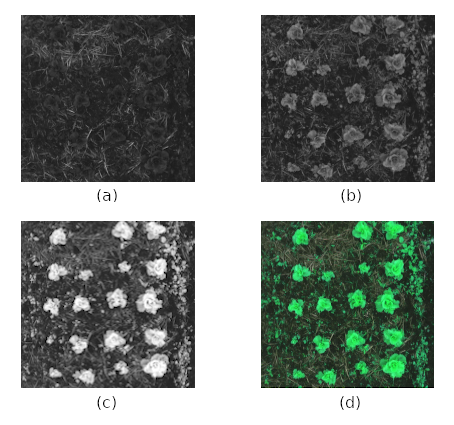
\includegraphics[scale=0.7]{dataset.png}
     \centering
    \caption{Dataset Images. (a) Red band 660nm. (b) Green band 550nm. (c) Near Infrared band 790nm. (d) Fake Green}
\end{figure}
\subsection{Method 1: HOG-SVM}
Las máquinas de soporte vectorial son modelos matemáticos cuyo objetivo principal es encontrar el hiperplano óptimo separador entre dos clases diferentes. Este paradigma se basa en un tipo de vectores conocidos como vectores de soporte que pueden estar en un espacio de dimensiones infinitas mapeados por medio de un kernel y un parámetro de coste\cite{c55}. En este caso se utilizaron los histogramas de gradiente orientado (HOG) como técnica que extrae las carácterísticas presentes en cada objeto de la imagen. Posteriormente se realizó un entrenamiento con un kernel polinómico utilizando 1400 imágenes de acuerdo al resultado principal obtenido en \cite{c4}. El objetivo principal de ete método es encontrar la clase (Maleza o lechuga) de un objeto determinado por una máscara creada a través del NDVI y el método de otsu. El diagrama de proceso se presenta en la imagen \ref{fig:svm_process} \cite{c4}.

Los histogramas de gradiente orientado son representaciones de un objeto en función de la magnitud y orientación del gradiente de un conjunto de bloques de pixeles determinados\cite{c4}. Este tipo de características permiten obtener la forma de una planta cuya geometría sea bien definida. En la figura \ref{fig:svm_process} se puede evidenciar el proceso de detección sin dejar atrás una fase de preprocesamiento utilizando el indice NDVI como estimador de fondo. Este indice se utiliza para crear una másacara que elimina objetos como el suelo y elementos que no tengan relación con la vegetación. Por otro lado se calculan los contornos de esta máscara y sus respectivas coordenadas son trasladas a la imagen original y asi obtener objetos con actividad fotosintética, estos objectos son sometidos a una extracción de caracteristicas por medio de histogramas de gradiente orientado que a su vez sirven como entrada a una maquina de soporte vectorial previamente entrenada. La SVM determinará si los objetos detectados pertenecen a la clase lechuga. Estos objetos pertenecientes a la clase previamente mencionada serán almacenados en una nueva máscara llamada mascara de cultivo ( ver figura \ref{fig:svm_process} Crop Mask).

Finalmente está máscara se multiplicará por la máscara obtenida por medio del índice NDVI eliminando a todos los objetos lechuga de la imagen quedando únicamente los objetos con acividad fotointética que son generalmente pertenecientes a las clase maleza. Finalmente a esta nueva máscara de maleza se le calculará el porcentaje de pixeles blancos respecto al área total de la imagen y de esta manera poder determinar su cobertura de maleza.

\begin{figure}[H]
    \centering
    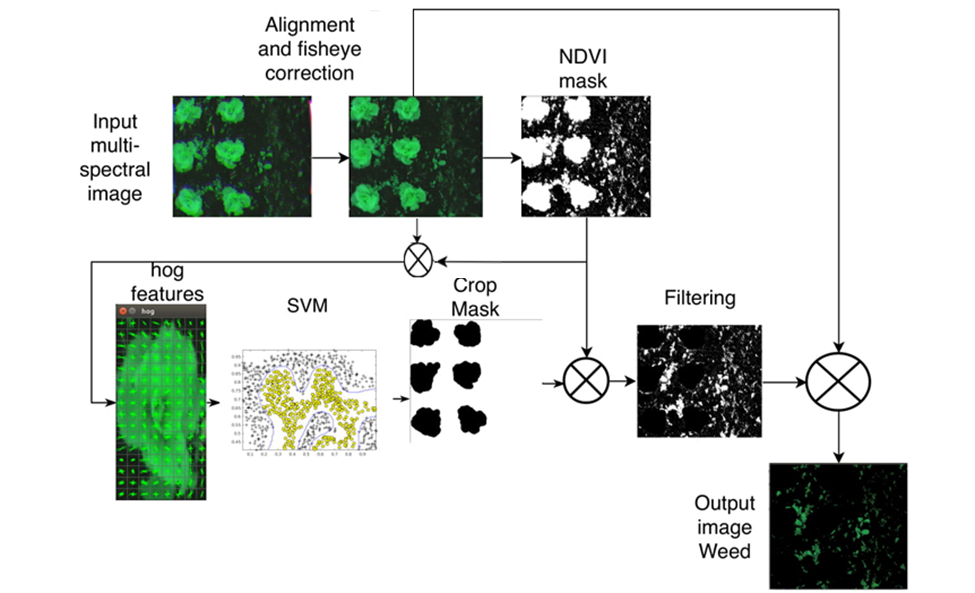
\includegraphics[scale=0.5]{svm_process}
     \centering
    \caption{Proceso utilizado en la detecció por medio de HOG-SVM. \label{fig:svm_process}\textcolor{correccion}{actualizar diagrama } }
\end{figure}

\subsection{Method 2: CNN - YOLOV3}
YOLO (You Look Only Once) como su nombre lo indica es una red neuronal capaz de detectar en una imagen los cuadros delimitadores de los objetos y la probabilidad de pertenencia de estos a una clase con solo un recorrido. La primera versión de YOLO salio en el 2016 \cite{c51}, su arquitectura constaba de 24 capas convolucionales que trabajan como extractores de características y dos capas densas o totalmente conectadas que realizan la predicción. En esta investigación, se trabajo con la versión tres YOLOv3 \cite{c53} la cual incluye mejoras significativas y las capas de extracción de características ya que fueron reemplazadas por la arquitectura Darknet-53 \cite{c53}.
\\
Como se observa en la Figura 2, (imagen c) en este método una vez el modelo esta entrenado para identificar el cultivo, un algoritmo localiza utiliza las coordenadas del bounding box arrojadas por el modelo para retirar las muestras de cultivo de la imagen, posteriormente se utiliza un filtro de verdes el cual binariza la imagen dejando negros los pixeles que no tienen vegetación mientras que los pixeles que pasaron el fitro de verdes son pintados con blanco resaltando así la vegetación que no corresponde al cultivo y simplificando el calculo porcentual de maleza por imagen.
\\
Con el fin de sacar el mayor provecho a YOLO en la detección de objetos y su velocidad se optó por no usar detección de bordes y  considerar como cultivo todo el bounding box generado por el modelo, aunque esto pudiera tener repercusiones en el calculo de maleza ya que se puede perder en la estimacion maleza mas proxima al cultivo.
\textcolor{correccion}{Agregar diagrama de METODO}

\subsection{Method 3: Mask R-CNN}
R-CNN usa el algoritmo selective search for object recognition \cite{c54} para extraer 2000 regiones de la imagen, estas alimentan una red neuronal convolucional en este caso Inception V2, la cual funciona como extractor de caracteristicas que se introducen a un SVM para que este clasifique el objeto segun la clase correspondiente. Ademas en este metodo al usar mascaras en el proceso de entrenamiento se obtendra una instance segmentation \cite{c56} la cual nos dara informacion detallada de los pixeles que pertenecen a la clase. 
El método de entrenamiento empleado en esta fase involucra un etiquetado del cultivo a manera de "bounding box" y un etiquetado de las máscara relacionada con cada clase. Esta máscara sale de la región cerrada correspondiente al cultivo que se encuentra dentro del "Bounding box" correspondiente. La arquitectura utilizada \cite{c56} permite acomodar las máscaras entrenadas previamente con la instancia detectada. Estas máscaras permiten obtener un contorno del objeto de interés sin tener que calcularlo como en el caso del método empleando SVM-HOG.\\
A diferencia de SVM-HOG, la estimación de la maleza se obtiene procesando inicialmente la imagen completa con la red convolucional. Esta red entregará las máscaras de cultivo correspondientes en una imagen binaria. Por otro lado el indice NDVI permite eliminar el fondo de la imagen dejando únicamete los objetos correspondientes a maleza y lechuga. Finalmente esta imagen se mezcla con la imagen de las máscaras generadas por la red neuronal para obtener finalmente una imagen de maleza. Finalmente se calcula el porcentaje de maleza presente en la imagen respecto al área total de la misma.
\textcolor{correccion}{ DIAGRAMA DEL METODO }
\begin{figure}[H]
    \centering
    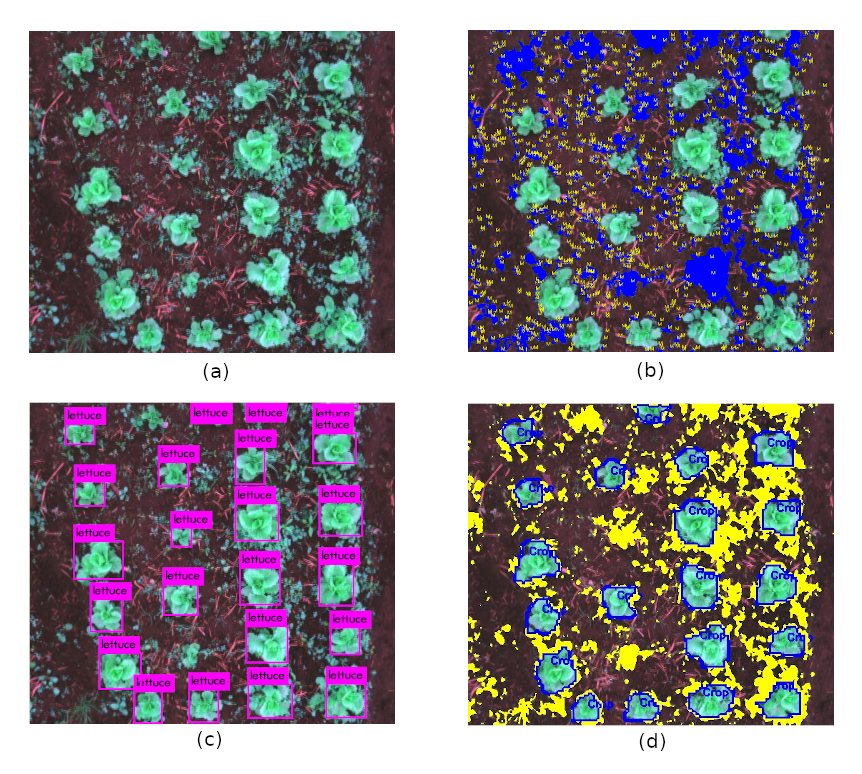
\includegraphics[scale=0.4]{Results.png}
     \centering
    \caption{ (a) Preprocessed image. (b) Method 1. (c) Method 2. (d) Method 3.}
\end{figure}
%%%%%%%%%%%%%%%%%%%%%%%%%%%%%%%%%%%%%%%%%%

\subsection{Experts evaluation}

En cuanto a la evaluación de los expertos se entrevistó a tres profesionales en malherbología, los cuales estimaron la cobertura de maleza en cada imagen. Es de resaltar que los profesionales tienen grados diferentes de formación: El experto 1 es B.sc en malherbología, el experto 2 es  M.sc en malherbología y el experto 3 es Ph.d en la misma área. Teniendo en cuenta que el 100\% corresponde a la totalidad de la imagen presentada y siendo evaluadas 100 imágenes, que posteriormente fueron procesadas por los métodos presentados previamente.

\subsection{Experimental setup}

Para este estudio se entrenaron tres modelos de cada método, los cuales fueron entrenados con 913 muestras etiquetadas manualmente por expertos. En el proceso de entrenamiento se utilizo una maquina con procesador Xeon de 8 núcleos, 16 GB de RAM y una gráfica GTX 1060 6GB. En la evaluación y comparación de desempeño, se selecciono el mejor modelo de cada metodo teniendo en cuenta sus matrices de confusion. Posteriormente se ejecutaron en ambientes separados con las mismas características: procesador Xeon 4 núcleos y 8GB de RAM, sin uso de tarjeta grafica. En cuanto a los lenguajes utilizados el método 1 se trabajo con C++, en el método 2 se utilizo el framework Darknet para entrenamiento y Python para evaluación, y para el método 3 se trabajo con python haciendo uso de la biblioteca TensorFlow.

\section{Results and Discussion}

En la tabla 2 se observan las métricas obtenidas por cada modelo en la cual se evidencia un buen desempeño de los tres modelos. Sin embargo  en este caso la exactitud no nos dice mucho ya que es un modelo evaluado bajo una sola clase y sin muestras negativas como lo evidencia la especificidad. Evaluando la sensibilidad y la precisión los modelos que usan YOLO y R-CNN se destacan con puntajes altos indicando que la predicción del cultivo fue muy acertada para estos modelos sin desmeritar el desempeño del modelo con HOG-SVM lo que se resume muy bien revisando el F1-Score de los tres modelos.

\begin{table}[H]
\centering
\caption{The performance evaluation of ML models in the training phase}
\begin{tabular}{|l|c|c|c|}
\hline
\multicolumn{1}{|c|}{\multirow{2}{*}{Training Metrics}} & \multicolumn{3}{c|}{Model} \\ \cline{2-4} 
\multicolumn{1}{|c|}{}                                  & HOG-SVM     & YOLO    & R-CNN  \\ \hline
Accuracy                                                & 79\%  & 89\%  & 89\% \\ \hline
Sensitivity                                             & 83\%  & 98\%  & 91\% \\ \hline
Specificity                                             & 0\%     & 0\%     & 0\%    \\ \hline
Precision                                               & 95\%  & 91\%    & 98\%   \\ \hline
F1-Score                                                & 88\%  & 94\%  & 94\% \\ \hline
\end{tabular}
\end{table}
\\



%\begin{figure}[H]
%    \centering
%    \includesvg[scale=0.7]{avg_time.svg}
%     \centering
%    \caption{Tiempo promedio de procesamiento por modelo}
%\end{figure}




Para comparar el tiempo empleado por cada uno de las técnicas, se revisó el uso de varios métodos no paramétricos (Nemenyi, Wilcox, Kruskal, Dunn) debido a la falta de normalidad, se escogió Wilcox, ya que los datos corresponden a muestras dependientes, de hecho son la misma población. Se encontró que existen diferencias estadísticas en el tiempo empleado entre los diferentes métodos. Sin embargo, en el boxplot (figura 5) se puede evidenciar que HOG-SVM y YOLO son más consistentes en el tiempo usado, mientras que RCNN, el tiempo que puede emplear es más variable.
\\
\begin{figure}[H]
    \centering
    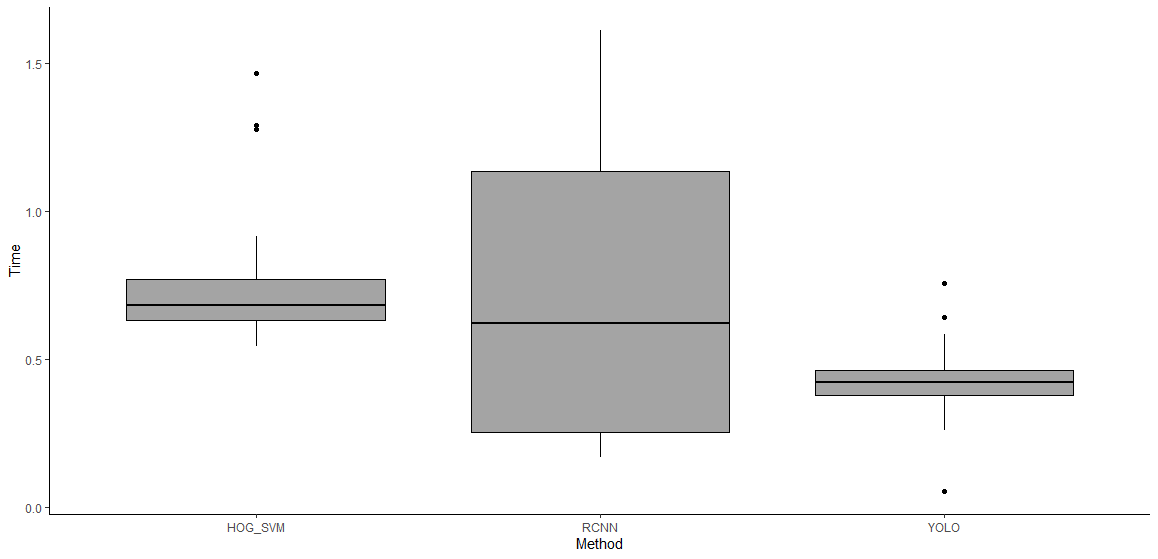
\includegraphics[scale=0.3]{boxplot1.png}
     \centering
    \caption{}
\end{figure}

Como lo menciona Ambrosio \cite{c3} a partir del muestreo con mallas cuadradas se determino que la densidad de las malezas como variable sigue una distribución de probabilidad binomial negativa, distribución que concuerda con las presentadas en la figura 5, lo cual indica que tanto la estimación de los modelos como la de los expertos se comportan según lo esperado, sin embargo si se analizan las curvas se pueden agrupar en tres grupos: el primero en el cual se encuentran los modelos que usaron HOG-SVM y RCNN los cuales presentan distribuciones parecidas y homogeneas con respecto a los demas. El segundo grupo que tiene al experto tres y al modelo entrenado con YOLO dado su comportamiento se puede decir que sus estimaciones tienen una tendencia similar. Por último en el tercer grupo se observa a los expertos uno y dos que tienen una distribución muy diferente respecto a los demás, pero similar entre ellos, lo que indica que sus datos tienden a una sobreestimar la cobertura con respecto a los demas, lo que evidencia que la subjetividad es uno de los principales problemas en la estimación de maleza realizada por humanos.

\begin{figure}[H]
    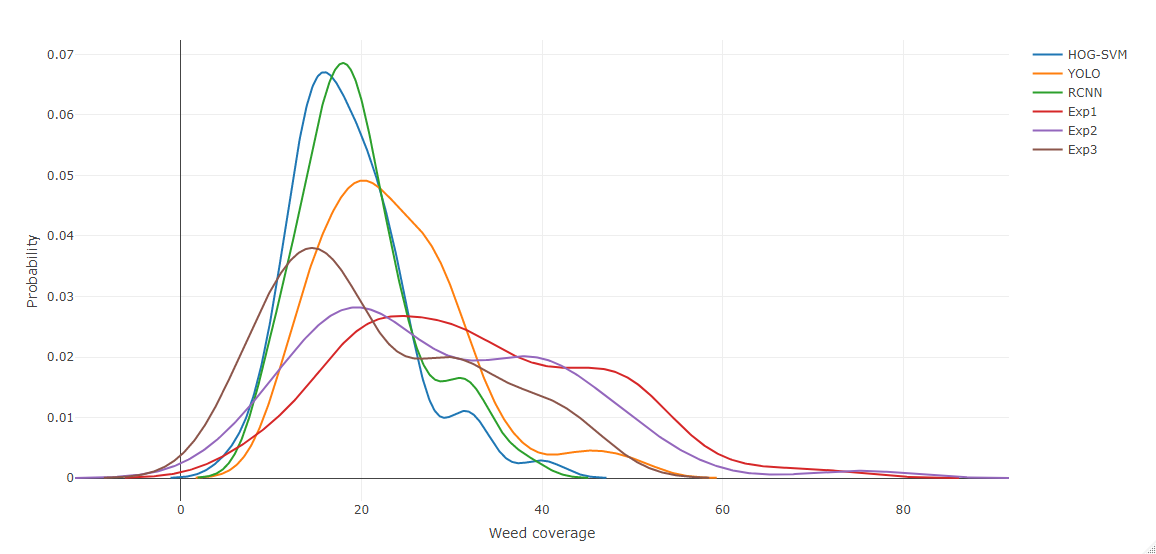
\includegraphics[scale=0.5]{weedcoveragedistribution.png}
    \caption{Weed coverage distribution}
\end{figure}

En cuanto al valor de cobertura se realizó un diagrama de cajas (Figure 7), para observar de forma exploratoria las posibles diferencias, luego se hizo el test de Dunn para comprobar la existencia de  diferencias significativas y finalmente, un análisis exploratorio para la comparación de correlacion y concordancia de los métodos con una matriz de correlación y graficos de bland altman.
\\
\begin{figure}[H]
    \centering
    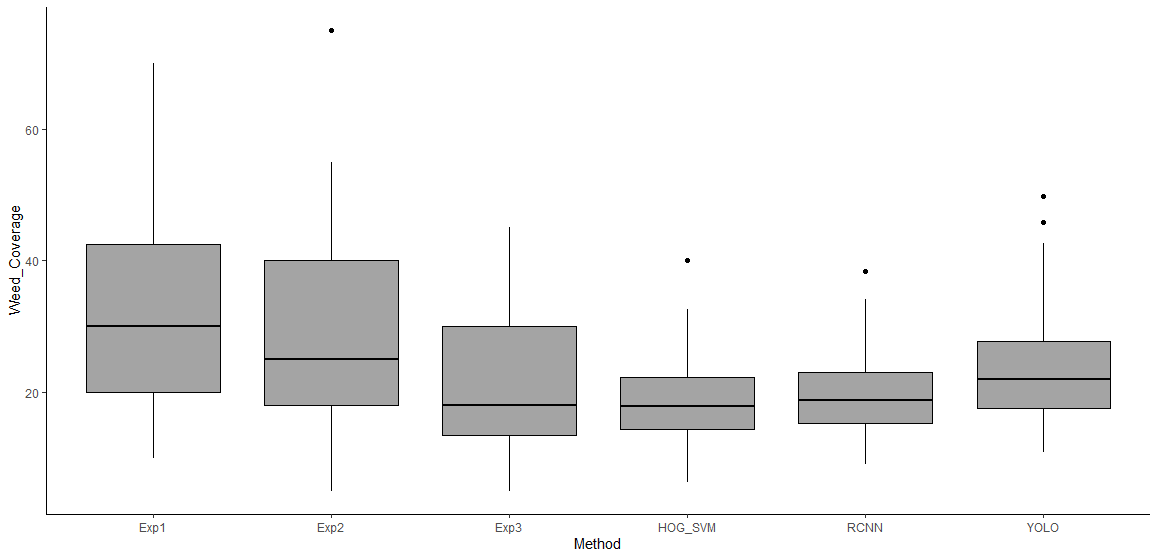
\includegraphics[scale=0.3]{boxplot2.png}
     \centering
    \caption{}
\end{figure}
\\
Se puede ver que RCNN y HOG-SVM son casi identicos, YOLO difiere un poco y se acerca mas a los expertos 1 y 2. Mientras que el experto 3 se encuentra cerca a RCNN y HOG-SVM, pero con una dispersión mayor de los datos. Los expertos 1 y 2, aumentan su dispersion debido a una mayor sobreestimacion de los valores más grandes de cobertura, como se observara con los graficos de Bland-Altman.
\begin{table}[H]
 \centering
 \caption{Matriz de valor-p, del test de Dunn.}
\begin{tabular}{|c|c|c|c|c|c|}
\hline
        & RCNN    & Exp1    & Exp2    & Exp3    & HOG-SVM \\ \hline
Exp1    & 8.7e-07 & -       & -       & -       & -       \\ \hline
Exp2    & 0.00430 & 0.45020 & -       & -       & -       \\ \hline
Exp3    & 0.99370 & 1.7e-05 & 0.02827 & -       & -       \\ \hline
HOG-SVM & 0.99405 & 3.5e-08 & 0.00048 & 0.87911 & -       \\ \hline
YOLO    & 0.25900 & 0.01379 & 0.69951 & 0.59922 & 0.07420 \\ \hline
\end{tabular}
\end{table}
Se puede ver que RCNN y HOG-SVM no tienen diferencias significativas con los otros dos métodos computacionales, ni con el experto 3. Que YOLO solo se diferencia de Exp1, que el exp 3 es estadísticamente diferente a los otros 2 expertos, pero no a ningún método computacional. Que el experto 2 es diferente a todos excepto a YOLO. Y que el experto uno es diferente a todos.
\\
Esto es explicado por la formación y nivel de entrenamiento, el experto 1, es un profesional de agronomía, pero con bajo entrenamiento en la cuantificación de coberturas de malezas, el profesional 2, es un profesional de agronomía con entrenamiento en la cuantificación de coberturas y el experto 3 es un doctor en agronomía con alto grado de entrenamiento. 

\begin{figure}[H]
    \centering
    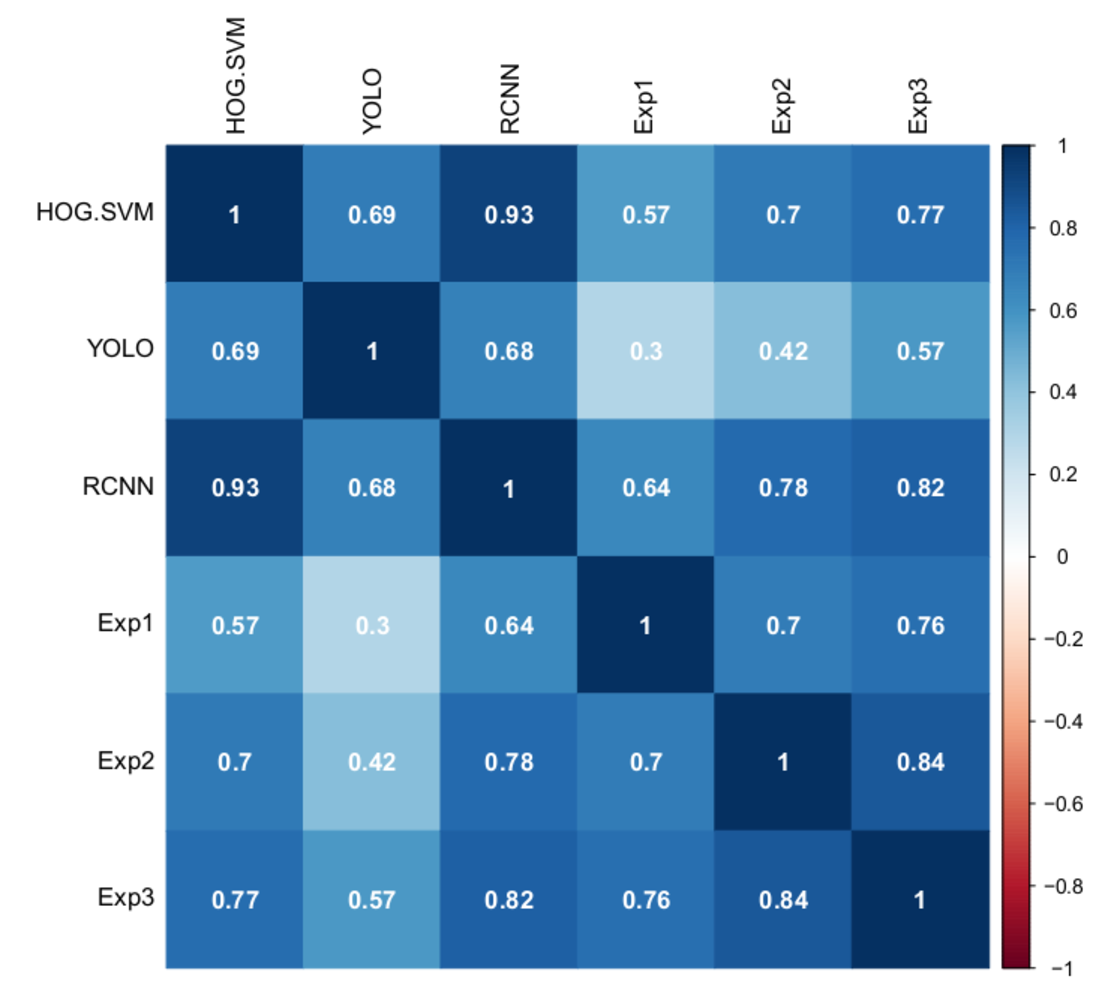
\includegraphics[scale=0.5]{corrmatrix.pdf}
     \centering
    \caption{Correlation matrix}
\end{figure}
En donde se evidencia que YOLO dentro de las técnicas computacionales y Exp1 dentro de los expertos, son los más inconsistentes.
\\
Comparar diferentes métodos de evaluación es una tarea compleja, ya que usualmente no se cuenta con un estándar o valor verdadero conocido. Entonces, una de las formas más usadas, pero a la vez más criticadas, es la correlación de Pearson, que evalúa asociación lineal entre las mediciones (variables), pero no evalúa su concordancia, por lo que dos métodos pueden correlacionarse bien, pero concordar poco, o viceversa \cite{c57}.
\\

La prueba de concordancia de Bland-Altman, permite encontrar límites de concordancia, sesgos y variabilidad. Por ejemplo en la figura 10 se compararon los métodos 1 y 3, se observa que los puntos no siguen ninguna distribución, que los límites de concordancia se encuentran entre -4 y +5 (situación que es tolerable en términos de las coberturas de las malezas), que el sesgo (línea azul) es casi paralela al eje x, aunque se puede corregir fácilmente y no hay sesgo de variabilidad, es decir, los datos no se dispersan más en la medida que aumentan los valores de cobertura. En conclusión cualquiera de los dos métodos pueden reemplazar al otro \cite{c59}.
\\
\begin{figure}[H]
    \centering
    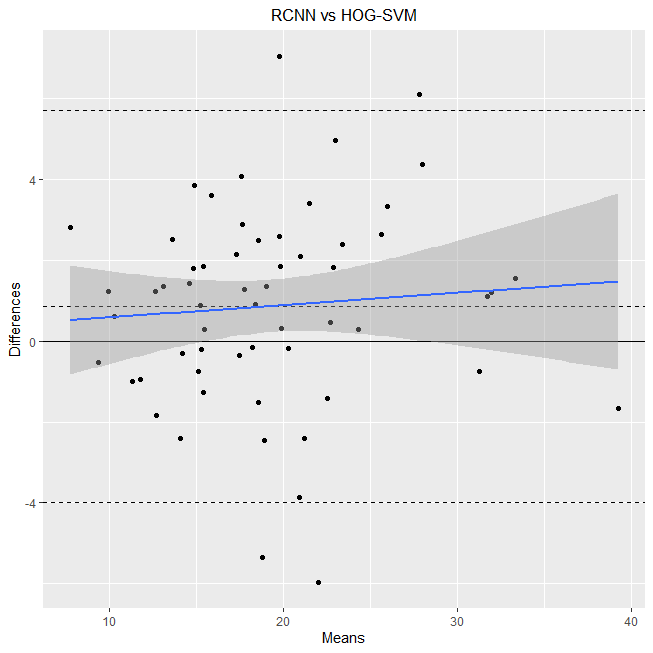
\includegraphics[scale=0.4]{RCNN-HOG-SVM.png}
     \centering
    \caption{}
\end{figure}
\\
Situación que cambia cuando se compara alguno de estos con el metodo 2, en donde a medida que aumenta la cobertura YOLO sobreestima la cobertura de las malezas, los límites de concordancia son más amplios (-15 hasta +10), y a medida que aumenta la cobertura, también aumenta la variabilidad de las diferencias.
\begin{figure}[H]
    \centering
    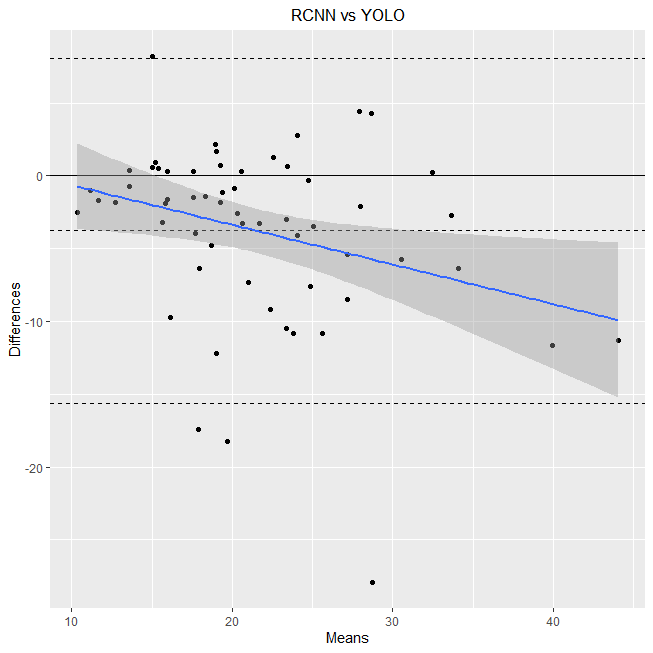
\includegraphics[scale=0.4]{RCNN-YOLO.png}
     \centering
    \caption{}
\end{figure}
\\
Cuando se compara el método computacional más consistente (Metodos 1 y 3), contra los valores obtenidos por los expertos, se puede corroborar la existencia del sesgo “humano”, es decir, se sobreestiman los valores altos de cobertura, en este caso hasta en 32 unidades de cobertura, Tambien, aumentan los límites de concordancia, desde -32 hasta 9. El promedio de los datos del experto 1 es mayor al del metodo 3 en 12 unidades de cobertura. Además, se puede ver que los expertos dan el dato redondeado en enteros o en múltiplos de 5 o 10, mientras que el método computacional da una variable continua. Finalmente, la precisión de los expertos no es buena, ya que para varias imágenes con un mismo valor de cobertura el experto uno, puede aumentar o disminuir el valor de cobertura en +- 10.
\begin{figure}[H]
    \centering
    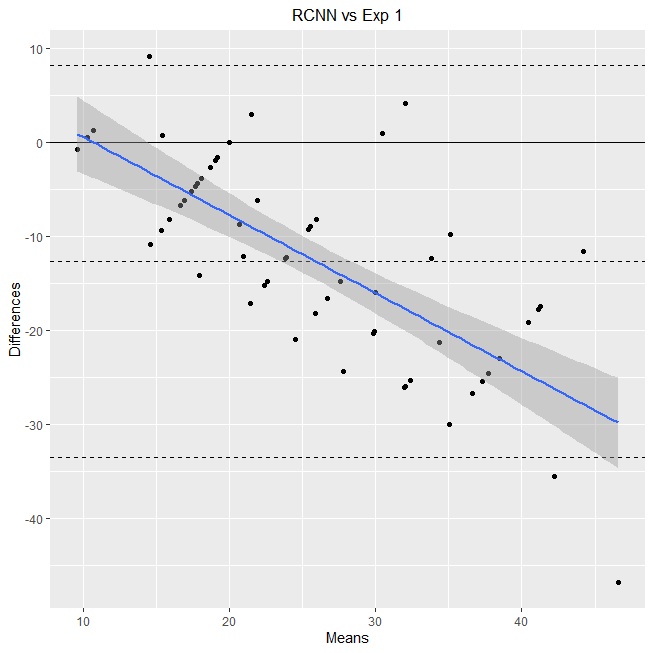
\includegraphics[scale=0.4]{RCNN-EXP1.png}
     \centering
    \caption{}
\end{figure}
\\
El experto 2, tuvo mayor precisión, los datos para un mismo valor de cobertura estuvieron en +-5 comparado con el metodo que uso RCNN, los límites de concordancia fueron ligeramente menores, desde -28 hasta + 8, sin embargo, también tiene el mismo sesgo en la sobreestimación de valores altos de cobertura.
\begin{figure}[H]
    \centering
    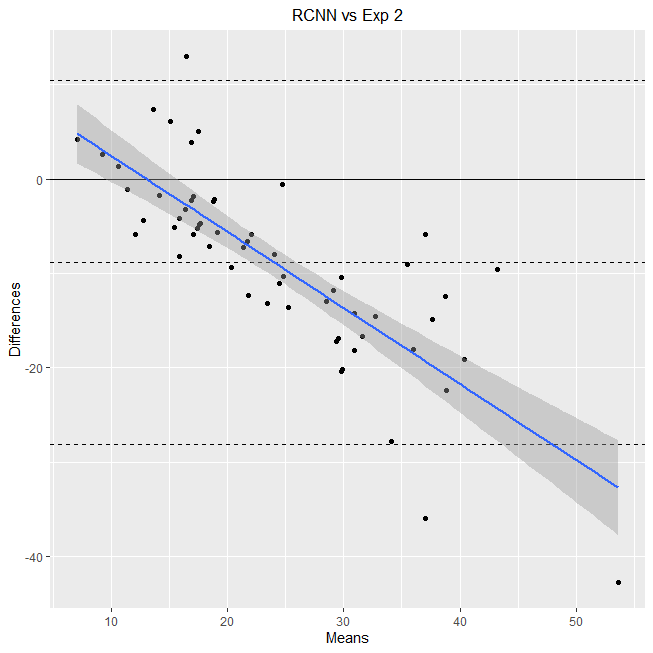
\includegraphics[scale=0.4]{RCNN-EXP2.png}
     \centering
    \caption{}
\end{figure}
\\
Para el experto 3, el rango de los límites de concordancia fue más bajo, desde -15 hasta +12, también presento el sesgo de sobreestimación pero en menor medida. Sin embargo, también subestimó los valores bajos de cobertura. Finalmente, no hubo sesgo de variabilidad y el valor promedio de la cobertura estuvo muy cerca del promedio del metodo 3.
\begin{figure}[H]
    \centering
    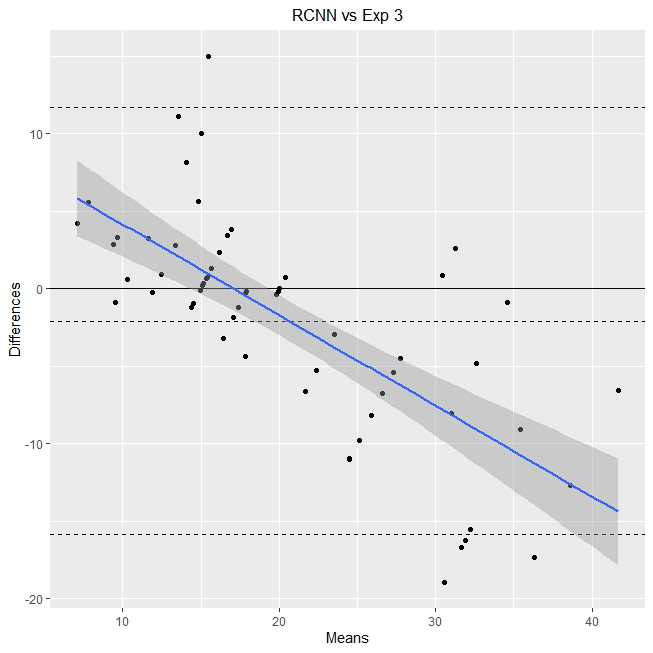
\includegraphics[scale=0.4]{RCNN-EXP3.png}
     \centering
    \caption{}
\end{figure}
\\
%%%%%%%%%%%%%%%%%%%%%%%%%%%%%%%%%%%%%%%%%%
\section{Conclusions}

La detección de maleza utilizando imágenes multiespectrales sigue siendo una tarea importante, ya que el control de estas es de vital importancia para la productividad agrícola. Por lo cual el desarrollo y mejoramiento de los métodos computacionales actuales es fundamental. Aunque el proceso puede ser difícil debido al establecimiento no uniforme y la carencia de características morfológicas distintivas para localizar la maleza, se ha visto una mejora significativa en cuanto a exactitud y velocidad en la detección de un cultivo en específico como tal, lo que permite distinguirlo del resto de la vegetación. 

La comparación de las estimaciones realizadas por profesionales y los modelos entrenados evidencia uno de los principales problemas que deben ser tratados utilizando aprendizaje automático en la agricultura de precisión como lo es el alto error que inserta la subjetividad del profesional en la estimación de maleza, lo que dificulta obtener un consenso acertado por profesionales y extiende el error a cálculos de horas de trabajo, cantidad y costo de materiales entre otros.
\\
Por lo anterior este trabajo presenta los modelos preentrenados para la estimación de maleza como una fuente fiable y con menos incertidumbre que puede ser adoptada por los profesionales dedicados al control de malezas.

El buen desempeño de los metodos se debe principalmente a como se abordo el problema de la estimación de maleza, fraccionandolo en diferentes problemas identificacion de la vegetacion, identificacion del cultivo y cuantificación. En principio se trabajo con dos clases maleza y cultivo teniendo muestras positivas y negativas de ambas clases, el problema radicó en la identificacion de la maleza debido a que posen pocas caracreristicas fijas su identificacion con los metodos empleados. Lo que generaba una elevada taza de error, por lo que se procedio a identificar la vegetacion usando bandas multiespectrales. Lo que dio oportunidad a que el modelo se concentrara en identificar unicamente el cultivo y asi facilitar al algoritmo el calculo de la vegetacion restante en este caso la maleza.

El modelo que uso YOLO llama la atención no solo por su velocidad si no que a pesar de que se tomaron los cultivos como rectangulos ignorando la maleza mas proxima al cultivo esto no afecto en gran medida a la estimacion con respecto a la evaluacion de los expertos, sin embargo el modelo R-CNN destaco por su exactitud a la hora de localizar el cultivo devolviendo su contorno de manera muy presisa metodo que puede ser recomendado para otros problemas del sector como la identificacion de frutos, en cuanto al metodo que uso HOG-SVM su deselmpeño fue muy bueno y teniendo en cuenta que necesita menor capacidad de procesamiento es una opcion muy buena para soluciones IoT.

Sin embargo la prueba de Bland Altan arrojo que los métodos basados en HOG-SVM y RCNN son los mas similares en cuanto a su evaluación, lo que permite determinarlos como los mas consistentes en la tarea, mientras que el método que uso YOLO sobrestima la cobertura de maleza de los valores altos con respecto a los otros dos. Ahora, si bien el sesgo humano de redondear los valores hace que sean menos precisos los expertos, al compararlos con los métodos 1 y 3 claramente existe sobrestimación y subestimación en los tres casos pero en diferente medida lo que indica que la variabilidad en la evaluación va ligada al grado de experiencia el experto y es tal vez, el problema mas grave que tiene la estimación visual humana. ya que al sobreestimar, se pueden tomar decisiones equivocadas de manejo. Pro ejemplo, un experto puede hallar el umbral de acción a nivel experimental, pero un evaluador de campo sobreestimara la cobertura y esto llevara a la realización de manejos no necesarios y al incremento e los gastos de producción y a una mayor contaminación.



%%%%%%%%%%%%%%%%%%%%%%%%%%%%%%%%%%%%%%%%%%
% Citations and References in Supplementary files are permitted provided that they also appear in the reference list here. 

%=====================================
% References, variant A: internal bibliography
%=====================================
\reftitle{References}
\begin{thebibliography}{999}

\bibitem{c1} Cheng, B., and Matson, E. T. (2015). A Feature-Based Machine Learning Agent for Automatic Rice and Weed Discrimination. Lecture Notes in Computer Science, 517–527.
\bibitem{c2} Wang, A., Zhang, W., and Wei, X. (2019). A review on weed detection using ground-based machine vision and image processing techniques. Computers and Electronics in Agriculture, 158, 226–240.
\bibitem{c3} Ambrosio, L., Iglesias, L., Marin, C., and Del Monte, J. (2004). Evaluation of sampling methods and assessment of the sample size to estimate the weed seedbank in soil, taking into account spatial variability. Weed Research, 44(3):224–236.
\bibitem{c4} Lara, A. E. P., Pedraza, C., & Jamaica-Tenjo, D. A. (2020). Weed Estimation on Lettuce Crops Using Histograms of Oriented Gradients and Multispectral Images. In Pattern Recognition Applications in Engineering (pp. 204-228). IGI Global.
\bibitem{c5} Hamuda, E., Mc Ginley, B., Glavin, M., and Jones, E. (2018). Improved image processing-based crop detection using Kalman filtering and the Hungarian algorithm. Computers and Electronics in Agriculture, 148, 37–44.
\bibitem{c6} Liakos, K. G., Busato, P., Moshou, D., Pearson, S., and Bochtis, D. (2018, August 14). Machine learning in agriculture: A review. Sensors (Switzerland). MDPI AG.
\bibitem{c7} López-Granados, F. (2011). Weed detection for site-specific weed ma- nagement: mapping and real-time approaches. Weed Research, 51(1):1–11
\bibitem{c8} Pantazi, X.E.; Tamouridou, A.A.; Alexandridis, T.K.; Lagopodi, A.L.; Kashefi, J.; Moshou, D. Evaluation of hierarchical self-organising maps for weed mapping using UAS multispectral imagery. Comput. Electron. Agric. 2017, 139, 224–230.
\bibitem{c9} Pantazi, X.-E.; Moshou, D.; Bravo, C. Active learning system for weed species recognition based on hyperspectral sensing. Biosyst. Eng. 2016, 146, 193–202.
\bibitem{c10} Binch, A.; Fox, C.W. Controlled comparison of machine vision algorithms for Rumex and Urtica detection in grassland. Comput. Electron. Agric. 2017, 140, 123–138.
\bibitem{c11} Xinshao, W., Cheng, C., 2015. Weed seeds classification based on PCANet deep learning baseline. IEEE Signal and Information Processing Association Annual Summit and Conference (APSIPA), pp. 408–415.
\bibitem{c12} Dyrmann, M., Mortensen, A.K., Midtiby, H.S., Jørgensen, R.N., 2016. Pixel-wise
classification of weeds and crops in images by using a fully convolutional neural network. International Conference on Agricultural Engineering. Aarhus, Denmark.
\bibitem{c13} Xinshao, W., Cheng, C., 2015. Weed seeds classification based on PCANet deep learning baseline. IEEE Signal and Information Processing Association Annual Summit and Conference (APSIPA), pp. 408–415.
\bibitem {c14}McCool, C., Pérez, T., Upcroft, B., 2017. Mixtures of lightweight deep convolutional neural networks: applied to agricultural robotics. IEEE Rob. Autom. Lett. 2 (3), 1344–1351.
\bibitem{c15} Dyrmann, M., Jørgensen, R.N., Midtiby, H.S., 2017. RoboWeedSupport – Detection of weed locations in leaf occluded cereal crops using a fully convolutional neural network. 11th European Conference on Precision Agriculture (ECPA). Edinburgh, Scotland
\bibitem{c16} Milioto, A., Lottes, P., Stachniss, C., 2017. Real-time blob-wise sugar beets vs weeds classification for monitoring fields using convolutional neural networks. Proceedings of the International Conference on Unmanned Aerial Vehicles in Geomatics. Bonn, Germany
\bibitem{c17} Potena, C., Nardi, D., Pretto, A., 2016. Fast and accurate crop and weed identification with summarized train sets for precision agriculture. In: International Conference on Intelligent Autonomous Systems. Springer, Cham, Shanghai, China, pp. 105–121.
\bibitem{c18} Dyrmann, M., Jørgensen, R.N., Midtiby, H.S., 2017. RoboWeedSupport – Detection of weed locations in leaf occluded cereal crops using a fully convolutional neural net- work. 11th European Conference on Precision Agriculture (ECPA). Edinburgh, Scotland
\bibitem{c19} Peña, J. M., Torres-Sánchez, J., de Castro, A. I., Kelly, M., and López-Granados, F. (2013). Weed Mapping in Early-Season Maize Fields Using Object-Based Analysis of Unmanned Aerial Vehicle (UAV) Images. PLoS ONE, 8(10), e77151. doi:10.1371/journal.pone.0077151
\bibitem{c20} Tellaeche, A., Burgos Artizzu, X. P., Pajares, G., Ribeiro, A., and Fernández-Quintanilla, C. (2008). A new vision-based approach to differential spraying in precision agriculture. Computers and Electronics in Agriculture, 60(2), 144–155.
\bibitem{c21} Rumpf, T., Römer, C., Weis, M., Sökefeld, M., Gerhards, R., and Plümer, L. (2012). Sequential support vector machine classification for small-grain weed species discrimination with special regard to Cirsium arvense and Galium aparine. Computers and Electronics in Agriculture, 80, 89–96.
\bibitem{c22} Nieuwenhuizen, A. T., Tang, L., Hofstee, J. W., Müller, J., and van Henten, E. J. (2007). Colour based detection of volunteer potatoes as weeds in sugar beet fields using machine vision. Precision Agriculture, 8(6), 267–278. 
\bibitem{c23} Milioto, A., Lottes, P., Stachniss, C., 2017. Real-time blob-wise sugar beets vs weeds classification for monitoring fields using convolutional neural networks. Proceedings of the International Conference on Unmanned Aerial Vehicles in Geomatics. Bonn, Germany.
\bibitem{c24} Hung, C., Xu, Z., and Sukkarieh, S. (2014). Feature learning based approach for weed classification using high resolution aerial images from a digital camera mounted on a UAV. Remote Sensing, 6(12), 12037–12054.
\bibitem{c25} Partel, V., Charan Kakarla, S., and Ampatzidis, Y. (2019). Development and evaluation of a low-cost and smart technology for precision weed management utilizing artificial intelligence. Computers and Electronics in Agriculture, 157(November 2018), 339–350.
\bibitem{c26} Pantazi, X. E., Tamouridou, A. A., Alexandridis, T. K., Lagopodi, A. L., Kashefi, J., and Moshou, D. (2017). Evaluation of hierarchical self-organising maps for weed mapping using UAS multispectral imagery. Computers and Electronics in Agriculture, 139, 224–230.
\bibitem{c27} López-Granados, F., Torres-Sánchez, J., Serrano-Pérez, A., de Castro, A. I., Mesas-Carrascosa, F. J., and Peña, J. M. (2016). Early season weed mapping in sunflower using UAV technology: variability of herbicide treatment maps against weed thresholds. Precision Agriculture, 17(2), 183–199.
\bibitem{c28} López-Granados, F., Torres-Sánchez, J., De Castro, A.-I., Serrano-Pérez, A., Mesas-Carrascosa, F.-J., and Peña, J.-M. (2016). Object-based early monitoring of a grass weed in a grass crop using high resolution UAV imagery. Agronomy for Sustainable Development, 36(4).
\bibitem{c29} Ahmed, O. S., Shemrock, A., Chabot, D., Dillon, C., Williams, G., Wasson, R., and Franklin, S. E. (2017). Hierarchical land cover and vegetation classification using multispectral data acquired from an unmanned aerial vehicle. International Journal of Remote Sensing, 38(8–10), 2037–2052.
\bibitem{c30} Huang, H., Deng, J., Lan, Y., Yang, A., Deng, X., and Zhang, L. (2018). A fully convolutional network for weed mapping of unmanned aerial vehicle (UAV) imagery. PLoS ONE, 13(4).
\bibitem{c31} Rojas, D., Gonzalez, C., and Perdomo, S. (2016). Weed Detection in Rice Fields Using Aerial Images and Neural Networks Faculty of Engineering e Faculty of Engineering Faculty of Engineering. IEEE Xplore.Universidad de Ibagué. 
\bibitem{c32} Chavan, T. R., and Nandedkar, A. V. (2018). AgroAVNET for crops and weeds classification: A step forward in automatic farming. Computers and Electronics in Agriculture, 154(September), 361–372.
\bibitem{c33} Sun, J., He, X., Ge, X., Wu, X., Shen, J., and Song, Y. (2018). Detection of Key Organs in Tomato Based on Deep Migration Learning in a Complex Background. Agriculture, 8(12), 196.
\bibitem{c34} Sa, I., Popovic, M., Khanna, R., Chen, Z., Lottes, P., Liebisch, F., … Siegwart, R. (2018). WeedMap: A large-scale semantic weed mapping framework using aerial multispectral imaging and deep neural network for precision farming.
\bibitem{c35} Huang, H., Lan, Y., Deng, J., Yang, A., Deng, X., Zhang, L., and Wen, S. (2018). A semantic labeling approach for accurate weed mapping of high resolution UAV imagery. Sensors (Switzerland), 18(7).
\bibitem{c36} Suh, H. K., IJsselmuiden, J., Hofstee, J. W., and van Henten, E. J. (2018). Transfer learning for the classification of sugar beet and volunteer potato under field conditions. Biosystems Engineering, 174, 50–65.
\bibitem{c37} Dyrmann, M., Karstoft, H., and Midtiby, H. S. (2016). Plant species classification using deep convolutional neural network. Biosystems Engineering, 151(2005), 72–80.
\bibitem{c38} Huang, H., Deng, J., Lan, Y., Yang, A., Deng, X., Wen, S., … Zhang, Y. (2018). Accurate weed mapping and prescription map generation based on fully convolutional networks using UAV imagery. Sensors (Switzerland), 18(10).
\bibitem{c39} Sa, I., Chen, Z., Popovic, M., Khanna, R., Liebisch, F., Nieto, J., and Siegwart, R. (2018). WeedNet: Dense Semantic Weed Classification Using Multispectral Images and MAV for Smart Farming. IEEE Robotics and Automation Letters, 3(1), 588–595.
\bibitem{c40} Kamilaris, A., and Prenafeta-Boldú, F. X. (2018). Deep learning in agriculture: A survey. Computers and Electronics in Agriculture, 147(February), 70–90.
\bibitem{c41}Srinivasan A (2006) Precision Agriculture: An Overview. In: A Srinivasan. Handbook of Precision Agriculture: Principles and Applications. New York: Food Products Press, The Haworth Press. pp. 3-18.
\bibitem{c42} Koger CH, Shaw DR, Watson CE, Reddy KN (2003) Detecting late- season weed infestations in soybean (Glycine max). Weed Technol 17: 696-704.
\bibitem{c43}Tao, T., Wu, S., Li, L., Li, J., Bao, S., and Wei, X. (2018). Design and experiments of weeding teleoperated robot spectral sensor for winter rape and weed identification. Advances in Mechanical Engineering, 10(5).
\bibitem{c44}L Xue, W Cao, W Luo, X Zhang,(2004).Correlation between leaf nitrogen status and canopy spectral characteristics in wheat. Acta Phytoecologica Sinica 28(2), 172-177.
\bibitem{c45}Bell, G..E., Howell, B..M., Johnson, G..V., Raun, W..R., Solie, J..B., and Stone, M..L. (2004). Optical Sensing of Turfgrass Chlorophyll Content and Tissue Nitrogen, HortScience HortSci, 39(5), 1130-1132.
\bibitem{c46}Behmann, J., Mahlein, A. K., Rumpf, T., Römer, C., and Plümer, L. (2015). A review of advanced machine learning methods for the detection of biotic stress in precision crop protection. Precision Agriculture, 16(3), 239–260. 
\bibitem{c47}B, F. S., Toshevska, M., and Gievska, S. (2018). Review of Automated Weed Control Approaches: An Environmental Impact Perspective (Vol. 940).
\bibitem{c48}Kharuf G, Hernández S, Orozco M, Aday D, Osmany de la C, y Delgado M,. (2018). Análisis de imágenes multiespectrales adquiridas con vehículos aéreos no tripulados. Ingeniería Electrónica, Automática y Comunicaciones, 39(2), 79-91
\bibitem{c49}Thorp, K. R., and Tian, L. F. (2004). A review on remote sensing of weeds in agriculture. Precision Agriculture, 5(5), 477–508.
\bibitem{c50} Brown, R. B., and Noble, S. D. (2005). Site-Specific Weed Management : Sensing Requirements : What Do We Need to See ? Published by : Weed Science Society of America and Allen Press Linked references are available on JSTOR for this article : Symposium Site-specific weed management : sensing re. 53(2), 252–258.
\bibitem{c51}Redmon J., Divvala S., Girshick R. and Farhadi A., 2016. You only look once: Unified,real-time object detection. In:The IEEE Conference on Computer Vision and Pattern Recognition (CVPR), pp. 779-788.
\bibitem{c52} Redmon J.,J. Redmon. Darknet: Open source neural networks in c. http://pjreddie.com/darknet/, 2013–2016.
\bibitem{c53}  J. Redmon and A. Farhadi. Yolov3: An incremental improvement. CoRR, abs/1804.02767, 2018.
\bibitem{c54}  Uijlings, J.R.R., van de Sande, K.E.A., Gevers, T. et al. Selective Search for Object Recognition. Int J Comput Vis 104, 154–171, 2013.
\bibitem{c55} Mountrakis, G., Im, J., & Ogole, C. (2011). Support vector machines in remote sensing: A review. ISPRS Journal of Photogrammetry and Remote Sensing, 66(3), 247-259..
\bibitem{c56}He, K., Gkioxari, G., Dollár, P., & Girshick, R. (2017). Mask r-cnn. In Proceedings of the IEEE international conference on computer vision, 2961-2969.
\bibitem{c57}Altman DG, Bland JM. (1983) Measurement in medicine: the analysis of method comparison studies. Statistician, 32, 307-317.
\bibitem{c58}Jamaica David and Plaza Guido. Evaluation of various conventional methods for sampling weeds in potato and spinach crops. Agron. colomb. [online]. 2014, vol.32, n.1, pp.36-43. 
\bibitem{c59} Cardemil, Felipe. (2017). Comparison analysis and applications of the Bland-Altman method: correlation or agreement?. Medwave. 17.
\end{thebibliography}

% The following MDPI journals use author-date citation: Arts, Econometrics, Economies, Genealogy, Humanities, IJFS, JRFM, Laws, Religions, Risks, Social Sciences. For those journals, please follow the formatting guidelines on http://www.mdpi.com/authors/references
% To cite two works by the same author: \citeauthor{ref-journal-1a} (\citeyear{ref-journal-1a}, \citeyear{ref-journal-1b}). This produces: Whittaker (1967, 1975)
% To cite two works by the same author with specific pages: \citeauthor{ref-journal-3a} (\citeyear{ref-journal-3a}, p. 328; \citeyear{ref-journal-3b}, p.475). This produces: Wong (1999, p. 328; 2000, p. 475)

%=====================================
% References, variant B: external bibliography
%=====================================
%\externalbibliography{yes}
%\bibliography{your_external_BibTeX_file}

%%%%%%%%%%%%%%%%%%%%%%%%%%%%%%%%%%%%%%%%%%
%% optional
%\sampleavailability{Samples of the compounds ...... are available from the authors.}

%% for journal Sci
%\reviewreports{\\
%Reviewer 1 comments and authors’ response\\
%Reviewer 2 comments and authors’ response\\
%Reviewer 3 comments and authors’ response
%}

%%%%%%%%%%%%%%%%%%%%%%%%%%%%%%%%%%%%%%%%%%
\end{document}

